% !TEX root = ../../Diploma.tex
\section{Learning a New Behaviour}
\subsection{Training with a long period and high discount factor}
\begin{figure}[h]
	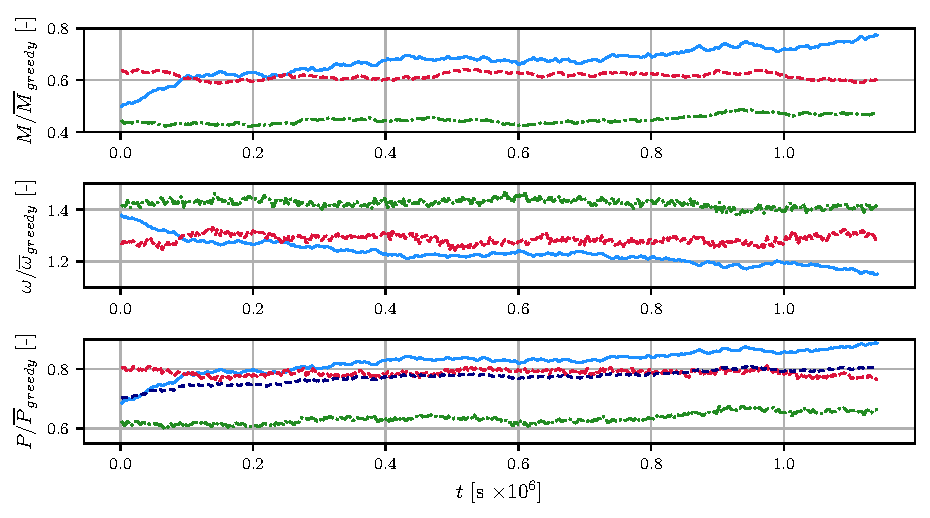
\includegraphics{plots/behaviour_optimization/torque_long_high_training.pdf}
	\caption{\legendFive{Turbine 0}{Turbine 1}{Turbine 2}{Total}{Greedy.} Training of agent with $\gamma=0.99$ and for periods with $N_{a,e}=1500$.}
	\label{fig:torque_long_high_training}
\end{figure} Since it could be shown, that the agent can improve the static parameters of a control strategy, the next step is to attempt to train an agent to learn a new behaviour. As described in \ref{ssec:new_behaviour_description}, three agents controlling the generator torque of the three turbines are trained. First, an agent with a long update period and a high discount factor will be examined. The long update period is chosen to allow the agent to develop lower frequency strategies. As was noted in \autoref{ssec:new_behaviour_description}, a high discount factor is chosen from an analysis of the physical timescales of the wind park. The timeseries of the generator torques, the angular velocities and the generated power of the three turbines as well as the total generated power are shown in \autoref{fig:torque_long_high_training}. It shows that after $\SI{1.2e6}{s}$ the performance by the agent is still significantly worse than that of a greedy controller. Therefore the training was stopped at this point. Furthermore, no improvement in total power is visible for $\SI{1e5}{s}$. The figure shows, that the torque of the first turbine is steadily increased throughout the training, while the torque of the second and third turbine show little change.
\begin{figure}[h]
	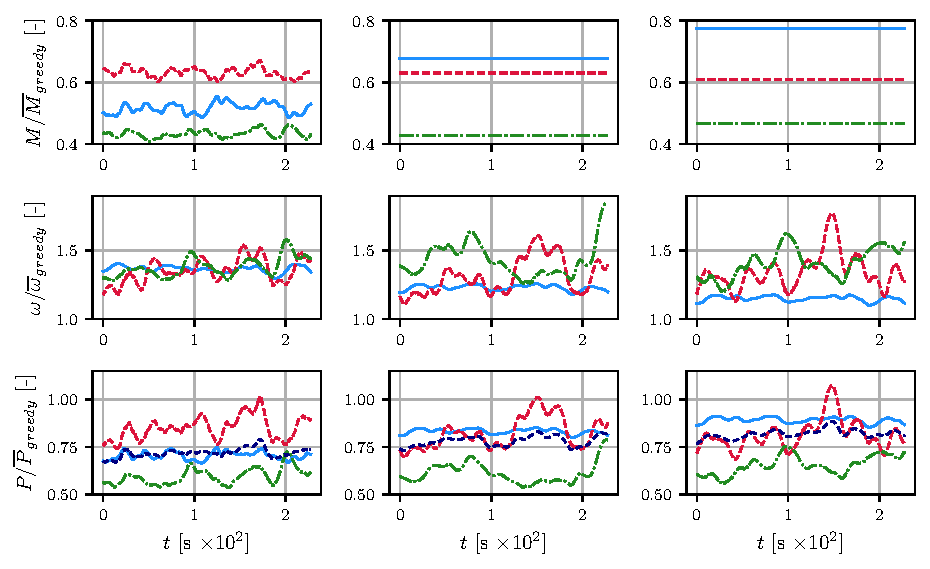
\includegraphics{plots/behaviour_optimization/torque_long_high_eval.pdf}
	\caption{\legendFive{Turbine 0}{Turbine 1}{Turbine 2}{Total}{Greedy.} Evolution of control strategy of agent with $\gamma=0.99$ and for periods with $N_{a,e}=1500$. Left column is control strategy in the beginning of training, central column after half of the training and right column after training has finished.}
	\label{fig:torque_long_high_eval}
\end{figure} \\
To analyze the evolution of the control strategy, despite it not being successful, \autoref{fig:torque_long_high_eval} shows generator torque, angular velocity and generated power by the turbines when controlled by the agent after 12 updates, after half of training time and after the full training time. The comparison of the control strategies shows that the agent evolves to set a constant generator torque at all three turbines. This is already visible after half of the training time. Furthermore, as was seen in \autoref{fig:torque_long_high_training}, the generator torque of the first turbine increases, while the torque at the other two turbines does not change after half of the training. A static generator torque differs from greedy control, but considering that the inflow has a uniform mean value, such a strategy still can be reasonable. However, since the total generated power only reached about three quarter of the total power of a greedy-controlled park, this strategy will not be investigated further. The major drawback of this agent was the slow evolution. One of the possible reasons for this is the long period between updates. Furthermore, the reason for the long period was the ability to develop lower frequency behaviour, which did not occur. Therefore another agent with a shorter update period was trained.
\subsection{Training with a short period and high discount factor}
\begin{figure}[h]
	\centering
	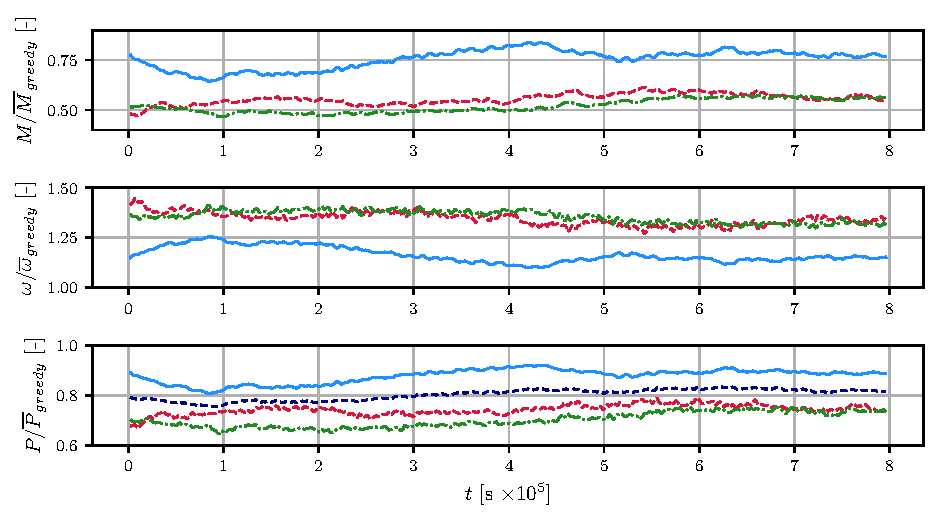
\includegraphics{plots/behaviour_optimization/torque_short_high_training.pdf}
	\caption{\legendFive{Turbine 0}{Turbine 1}{Turbine 2}{Total}{Greedy.} Training of agent with $\gamma=0.99$ and for periods with $N_{a,e}=500$.}
	\label{fig:torque_short_high_training}
\end{figure}
To increase the number of updates per simulated time, an agent with a number of actions per episode of 500 was trained. The timeseries of the generated power, angular velocity and generator torque are shown in \autoref{fig:torque_short_high_training}. It shows 
\begin{figure}[h]
	\centering
	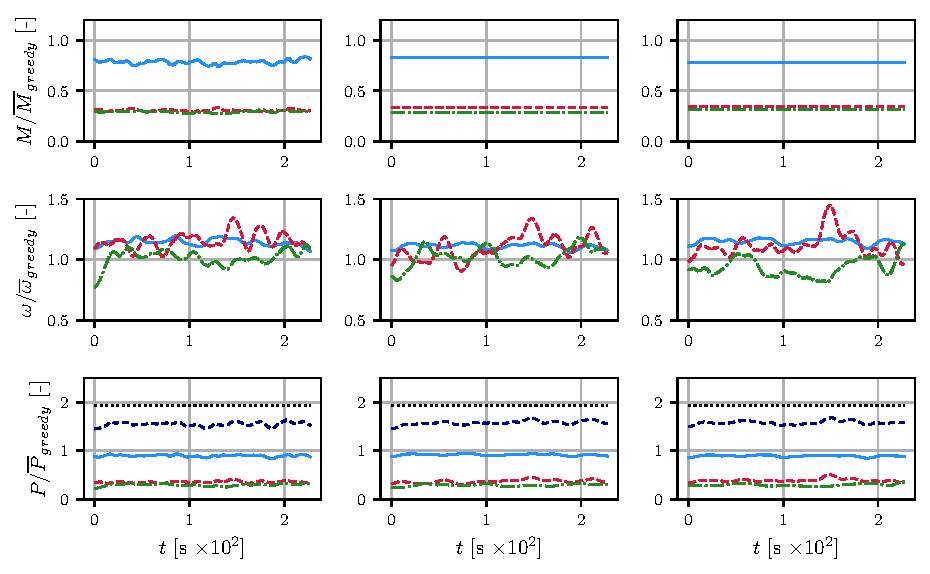
\includegraphics{plots/behaviour_optimization/torque_short_high_eval.pdf}
	\caption{\legendFive{Turbine 0}{Turbine 1}{Turbine 2}{Total}{Greedy.} Evolution of control strategy of agent with $\gamma=0.99$ and for periods with $N_{a,e}=500$. Left column is control strategy in the beginning of training, central column after half of the training and right column after training has finished.}
	\label{fig:torque_short_high_eval}
\end{figure}
\subsection{Training with a short period and low discount factor}
\begin{figure}[h]
	\centering
	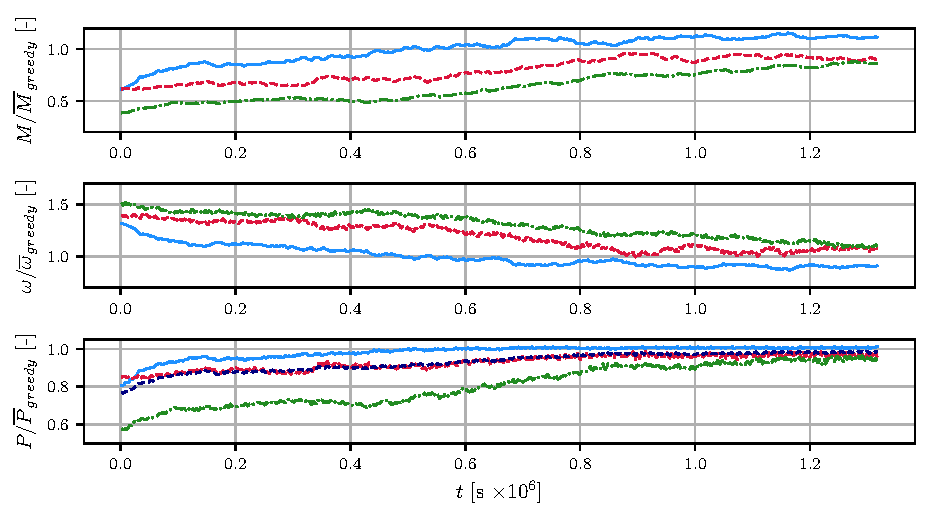
\includegraphics{plots/behaviour_optimization/torque_short_low_training.pdf}
	\caption{\legendFive{Turbine 0}{Turbine 1}{Turbine 2}{Total}{Greedy.} Training of agent with $\gamma=0.95$ and for periods with $N_{a,e}=500$.}
	\label{fig:torque_short_low_training}
\end{figure}
\begin{figure}[h]
	\centering
	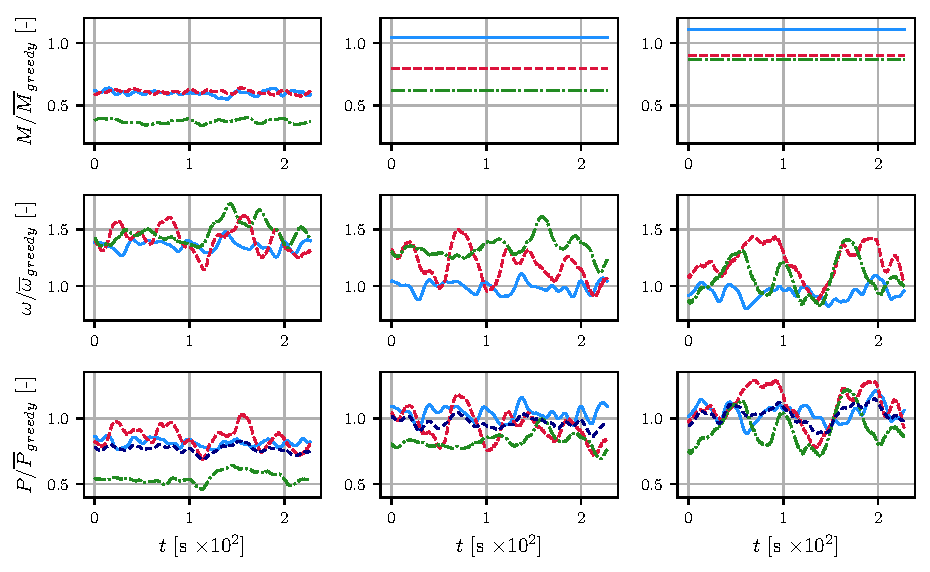
\includegraphics{plots/behaviour_optimization/torque_short_low_eval.pdf}
	\caption{\legendFive{Turbine 0}{Turbine 1}{Turbine 2}{Total}{Greedy.} Evolution of control strategy of agent with $\gamma=0.95$ and for periods with $N_{a,e}=500$. Left column is control strategy in the beginning of training, central column after half of the training and right column after training has finished.}
	\label{fig:torque_short_low_eval}
\end{figure}
\subsection{Analysis of flow}
\begin{table}[h]
	\centering
	\caption{Mean, relative difference in mean and relative in standard deviation of power and aerodynamic moment of a trained torque-controlling agent in comparison to the greedy-control case.}
	\begin{tabular}{ccccccc}
		\toprule
		& \multicolumn{3}{c}{$P$}  & \multicolumn{3}{c}{$M_{aero}$ }\\ \cmidrule(rl){2-4} \cmidrule(rl){5-7}
		& mean & rel. mean & rel. std  & mean & rel. mean & rel. std \\ \midrule
		Total & $\SI{  9.65}{MW} $ & $\SI{ -1.42}{\%}$ & $\SI{ -19.3}{\%}$ &-&-&- \
		\\
		Turbine 0  & $\SI{   5.1}{MW} $ & $\SI{+0.837}{\%}$ & $\SI{ +6.28}{\%}$ & $\SI{3.53e03}{kNm} $ & $\SI{ +10.6}{\%}$ & $\SI{ +14.8}{\%}$ \\
		Turbine 1  & $\SI{  2.48}{MW} $ & $\SI{ -3.23}{\%}$ & $\SI{ -22.5}{\%}$ & $\SI{1.82e03}{kNm} $ & $\SI{ -9.65}{\%}$ & $\SI{ -4.19}{\%}$ \\
		Turbine 2  & $\SI{  2.07}{MW} $ & $\SI{ -4.55}{\%}$ & $\SI{ -26.1}{\%}$ & $\SI{1.57e03}{kNm} $ & $\SI{ -13.2}{\%}$ & $\SI{ -6.25}{\%}$ \\
		\bottomrule
	\end{tabular}
\end{table}
\begin{figure}[h]
	\centering
	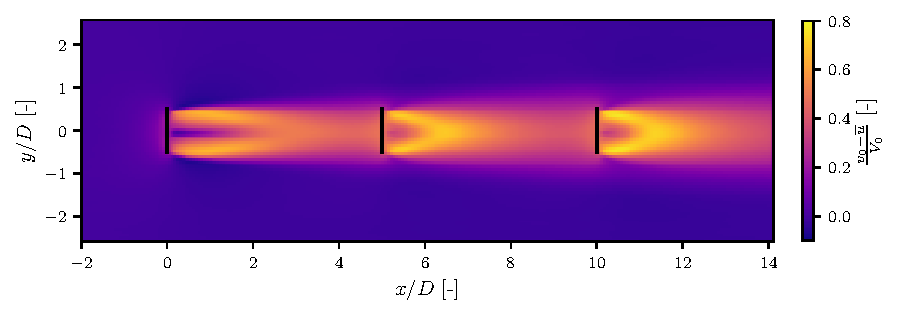
\includegraphics{plots/behaviour_optimization/torque_short_low_velocity.pdf}
	\caption{{\color{black} \rule[3pt]{22pt}{1pt} Turbine.} Turbulence intensity of optimized helix control.}
\end{figure}
\begin{figure}[h]
	\centering
	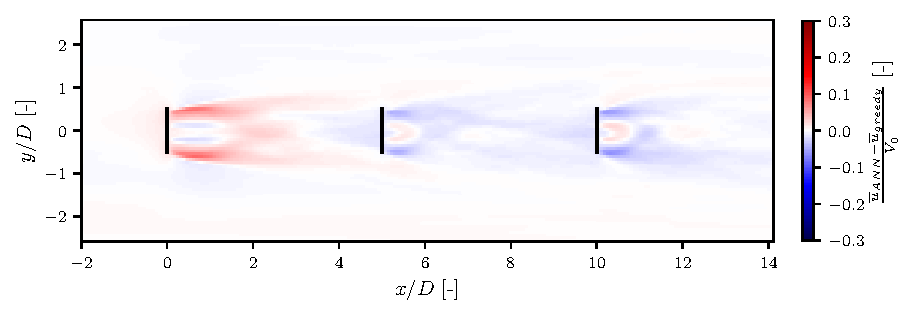
\includegraphics{plots/behaviour_optimization/torque_short_low_velocity_difference.pdf}
	\caption{{\color{black} \rule[3pt]{22pt}{1pt} Turbine.} Turbulence intensity of optimized helix control.}
\end{figure}
\begin{figure}[h]
	\centering
	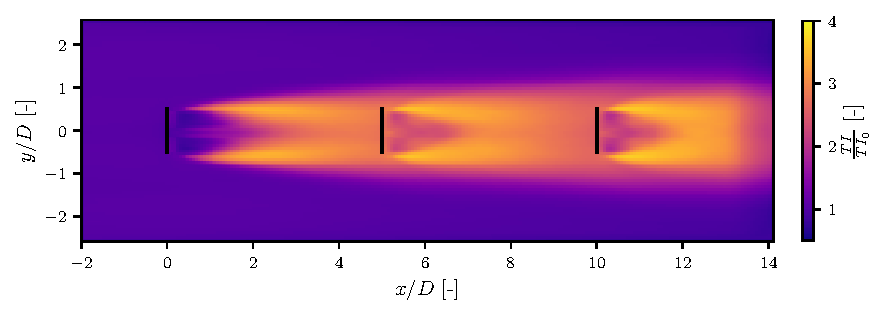
\includegraphics{plots/behaviour_optimization/torque_short_low_turbulence_intensity.pdf}
	\caption{{\color{black} \rule[3pt]{22pt}{1pt} Turbine.} Turbulence intensity of optimized helix control.}
\end{figure}
\begin{figure}[h]
	\centering
	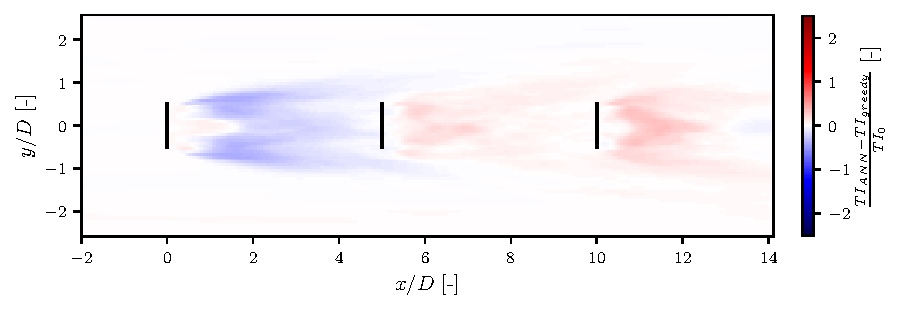
\includegraphics{plots/behaviour_optimization/torque_short_low_ti_difference.pdf}
	\caption{{\color{black} \rule[3pt]{22pt}{1pt} Turbine.} Turbulence intensity of optimized helix control.}
\end{figure}